\documentclass[a4paper,11pt]{article}
\usepackage[T1]{fontenc}
\usepackage[utf8]{inputenc}
\usepackage[italian]{babel}
% LAYOUT
\usepackage{geometry}
	\geometry{a4paper,top=2cm,bottom=2cm,
	left=2.5cm,right=2.5cm,heightrounded}
\usepackage[backend=biber,style=numeric,hyperref]{biblatex}
	\addbibresource{bibliografia.bib}
\usepackage{booktabs,array}
\usepackage{caption,subcaption}
	\captionsetup{tableposition=top,figureposition=bottom}
	\captionsetup{justification=centering,font=small,labelfont=bf}
\usepackage{hyperref}
	\hypersetup{hidelinks}
\usepackage{microtype}
% SCIENTIFIC TYPESETTING
\usepackage{amsmath, amsthm, amssymb, mathtools}
\usepackage{bm, mathrsfs}
\usepackage{siunitx}
\usepackage{resizegather}
	\addtolength{\jot}{4pt}
\usepackage{pythonhighlight}

\renewcommand{\vec}[1]{\bm{#1}}
\newcommand{\mat}[1]{\bm{#1}}
\newcommand{\tns}[1]{\bm{#1}}

\newcommand{\N}{\mathbb{N}}
\newcommand{\Z}{\mathbb{Z}}
\newcommand{\Q}{\mathbb{Q}}
\newcommand{\R}{\mathbb{R}}
\newcommand{\C}{\mathbb{C}}
\newcommand{\abs}[1]{\left\lvert#1\right\rvert}
\newcommand{\norm}[1]{\left\lVert#1\right\rVert}
\newcommand{\deq}{\vcentcolon=}
\newcommand{\eqd}{=\vcentcolon}
\newcommand{\dx}{\, dx}
\newcommand{\grad}{\nabla}
\renewcommand{\Re}{\operatorname{Re}}
\renewcommand{\Im}{\operatorname{Im}}
\newcommand{\code}[1]{\begin{small}\texttt{#1}\end{small}}

\DeclareMathOperator{\Ker}{Ker}
\DeclareMathOperator{\Rank}{Rank}
\DeclareMathOperator{\spn}{span} % \span è già utilizzato da latex
\DeclareMathOperator{\diver}{div}
\DeclareMathOperator{\supp}{supp}
\DeclareMathOperator{\TV}{TV}
\DeclareMathOperator{\tr}{tr}

\title{\Huge{\bf{
	Elaborato per il corso \\
	\emph{Methods for Parallel Programming}
}}}
\author{\huge{Bruno Degli Esposti}}
\date{\Large{Luglio/Agosto 2022}}

\begin{document}

\maketitle

\begin{abstract}
Questo elaborato descrive il processo di parallelizzazione
tramite MPI di un algoritmo iterativo per la soluzione di
sistemi lineari, il \emph{metodo del gradiente coniugato}.
Tale algoritmo viene applicato alla soluzione di un
boundary value problem monodimensionale tramite il metodo
delle differenze finite. Il codice è stato scritto in Python
e fa uso delle librerie \code{numpy} e \code{mpi4py}.
Sono stati effettuati test sulle proprietà di strong scaling
e weak scaling dell'algoritmo parallelo in esecuzione su
un cluster MPI domestico composto da due computer portatili
connessi tramite rete gigabit ethernet.
\end{abstract}

\section{Formulazione matematica del problema}
\subsection{Equazione di diffusione-reazione}
Sia $u(x)$ una quantità fisica (ad esempio, la concentrazione
di una specie chimica) definita in ogni punto di un dominio
monodimensionale $\Omega = [x_L,x_R]$. Se al variare del tempo
$u(x)$ è soggetta unicamente a processi di diffusione e di
reazione, la configurazione di equilibrio per tempi grandi
in presenza di un termine di sorgente/pozzo $f(x)$ è data
dalla soluzione del seguente boundary value problem (BVP):
\begin{equation} \label{eq:bvp}
\begin{cases}
-\mu(x) u''(x) + \sigma(x) u(x) = f(x)
& \text{per ogni $x \in (x_L,x_R)$} \\
u(x_L) = u_L \in \R \\
u(x_R) = u_R \in \R
\end{cases}
\end{equation}
Le condizioni al bordo $u(x_L) = u_L, u(x_R) = u_R$ sono dette
\emph{condizioni di Dirichlet} e corrispondono all'ipotesi che
la quantità $u(x)$ sia fissata agli estremi del dominio.
La funzione $\mu(x)$ è detta \emph{diffusività} del mezzo $\Omega$
ed è sempre strettamente positiva, quindi a meno di una divisione
per $\mu(x)$ possiamo supporre $\mu(x) \equiv 1$ senza perdita
di generalità.
La funzione $\sigma(x) \geq 0$ è detta \emph{tasso di reazione}
e sotto opportune ipotesi di regolarità per $\sigma(x)$ e $f(x)$
si può dimostrare che il problema \eqref{eq:bvp} ha soluzione
e che questa è unica.

\subsection{Metodo delle differenze finite}
Il \emph{metodo delle differenze finite} è una delle possibili
tecniche di discretizzazione esistenti in analisi numerica per
trasformare un'equazione differenziale come la \eqref{eq:bvp}
in un sistema di equazioni algebriche. In questo elaborato abbiamo
scelto di usare questo metodo per la sua semplicità sia
concettuale che di implementazione. L'idea fondamentale del
metodo delle differenze finite è quella di approssimare i valori
puntuali di $u(x)$ in un numero finito di ascisse $x_i$ distribuite
all'interno del dominio $\Omega$. Nel seguito indicheremo con
$u(x_i)$ il valore della soluzione esatta in $x_i$ e con $u_i$
la sua approssimazione numerica. Dunque le variabili $u_i$ saranno
le incognite del sistema di equazioni algebriche ottenuto dalla
discretizzazione di \eqref{eq:bvp}. Per semplicità, supponiamo
che le ascisse $x_i$ siano equispaziate:
\[
x_i = x_L + ih, \quad h = \frac{x_R-x_L}{N+1}, \quad i = 0,\dots,N+1
\]
Abbiamo dunque $N$ ascisse interne al dominio (da $x_1$ a $x_N$)
e due ascisse sul bordo del dominio ($x_0 = x_L$ e $x_{N+1} = x_R$).
La quantità $h$ è detta \emph{passo di discretizzazione}.
In ogni punto $x_i \in (x_L,x_R)$, la derivata seconda di $u$ si può
approssimare tramite differenze finite:
\begin{align} \label{eq:stencil}
u''(x_i)
&= \frac{u(x_i-h) - 2u(x_i) + u(x_i+h)}{h^2} + O(h^2) \\
&= \frac{u(x_{i-1}) - 2u(x_i) + u(x_{i+1})}{h^2} + O(h^2)
\end{align}
La dimostrazione è immediata utilizzando la formula di Taylor
per $u$ centrata in $x_i$. Dato che $u_i \approx u(x_i)$, la
valutazione dell'equazione \eqref{eq:bvp} nelle ascisse $x_i$
insieme alla formula \eqref{eq:stencil} suggeriscono lo
schema numerico
\begin{equation} \label{eq:fdm}
\begin{cases}
-(u_{i-1} - 2u_i + u_{i+1})h^{-2} + \sigma(x_i) u_i = f(x_i) \\
u_0 = u_L \\
u_{N+1} = u_R
\end{cases}
\end{equation}
Questo non è altro che un sistema lineare nell'incognita
vettoriale $\vec{u} = (u_1,\dots,u_N)^T$. Siano
\[
A = \frac{1}{h^2}
\begin{psmallmatrix}
2 & -1 &   &   &   &   &   \\ 
-1 & 2 & -1 &   &   &   &   \\ 
  & -1 & 2 & -1 &   &   &   \\ \vspace*{0.5em}
  &   & \ddots & \ddots & \ddots  &   &   \\
  &   &   & -1 & 2 & -1 &   \\ 
  &   &   &   & -1 & 2 & -1 \\ 
  &   &   &   &   & -1 & 2
\end{psmallmatrix}
+
\begin{pmatrix}
\sigma(x_1) &  &  \\ 
  & \ddots &   \\ 
  &   & \sigma(x_N)
\end{pmatrix},
\qquad
\vec{b} = \begin{pmatrix}
f(x_1) + h^{-2} u_L \\ 
f(x_2) \\ 
\vdots \\ 
f(x_{N-1}) \\ 
f(x_N) + h^{-2} u_R
\end{pmatrix}.
\]
Allora il metodo delle differenze finite consiste nella
risoluzione del sistema lineare $A\vec{u} = \vec{b}$. Osserviamo che
la matrice $A$ è simmetrica. Si può dimostrare che $A$
è anche definita positiva.
Una volta risolto il sistema lineare, la qualità della soluzione
ottenuta si può valutare confrontando i valori numerici $u_i$ con
i valori esatti $u(x_i)$, supponendo di conoscere $u(x)$.
Soluzioni esatte $u(x)$ possono essere costruite
a tavolino assegnando funzioni arbitrarie a $u(x)$ e $\sigma(x)$
e scegliendo $f(x)$ di conseguenza (\emph{method of manufactured solutions}). In tutti i test numerici abbiamo scelto
\begin{equation} \label{eq:test-problem}
\begin{gathered}
x_L = 0, \quad
x_R = 1, \quad
u_L = 0, \quad
u_R = 0, \\
u(x) = \sin(\pi x), \quad
\mu(x) \equiv 1, \quad
\sigma(x) = \frac{1}{1+x^2}, \quad
f(x) = \left( \pi^2 + \frac{1}{1+x^2} \right) \sin(\pi x)
\end{gathered}
\end{equation}
e abbiamo stimato l'errore in norma infinito del metodo
numerico tramite l'indicatore
\[
e_\infty = \max_{i=1,\dots,N} \left\{ \abs{u_i - u(x_i)} \right\}.
\]
La regolarità dei dati $\sigma$ e $f$ permette di dimostrare
che il metodo delle differenze finite ha convergenza quadratica,
vale a dire che $e_\infty = O(h^2)$.

\subsection{Metodo del gradiente coniugato}
Nel paragrafo precedente ci siamo ricondotti alla soluzione
di un sistema lineare $A\vec{u} = \vec{b}$, con $A$ matrice
$N \times N$ simmetrica definita positiva (SDP).
Osserviamo che la matrice $A$ è sparsa, ossia che possiede
solo $O(N)$ termini non nulli anziché $O(N^2)$.
Per matrici sparse esistono algoritmi
ad hoc di tipo iterativo molto più efficienti in tempo
e in spazio dei classici algoritmi basati sulle fattorizzazioni
(come la fattorizzazione LU alla base dell'eliminazione gaussiana).
Nel caso di matrice simmetrica definita positiva sparsa
lo stato dell'arte è rappresentato dal \emph{metodo del
gradiente coniugato}.

Il metodo del gradiente coniugato, come molti altri metodi
iterativi per matrici SDP, sfrutta l'equivalenza tra il
problema della soluzione del sistema lineare
\[
A\vec{u} = \vec{b}
\]
e la minimizzazione della forma quadratica
\[
\Phi(\vec{u})
= \frac{1}{2} \vec{u}^T A \vec{u} - \vec{b}^T \vec{u} + c
\]
con $c$ costante arbitraria. È infatti immediato verificare
che $\grad \Phi(\vec{u}) = 0$ se e solo se $\vec{u} = A^{-1}\vec{b}$.
Il metodo del gradiente (semplice, non coniugato) è proprio
l'analogo metodo di \emph{gradient descent} ben noto
nell'ambito dell'ottimizzazione numerica, qui applicato alla
forma quadratica $\Phi$.
Osserviamo che $-\grad \Phi(\vec{u}) = \vec{b}-A\vec{u}$,
quindi il costo di
ogni iterazione è a grandi linee il costo di un prodotto
matrice-vettore, che grazie all'ipotesi di sparsità di $A$
ha costo computazionale $O(N)$ anziché $O(N^2)$.
Nell'ambito dei metodi iterativi per sistemi lineari,
la quantità $\vec{b}-A\vec{u}$ è detta \emph{residuo},
viene indicata con $\vec{r}$ ed è importante perché fornisce
un'indicazione di quanto il vettore $\vec{u}$ sia lontano dal
risolvere il sistema lineare $A\vec{u} = \vec{b}$.
Notiamo come in questo contesto antigradiente e residuo coincidano.

Sia $\vec{u}_0$ un vettore arbitrario in $\R^N$.
Durante la prima iterazione, il metodo del gradiente
coniugato si comporta esattamente come il metodo del
gradiente semplice: la direzione di discesa $\vec{p}_0$
è uguale al residuo $\vec{r}_0$, e la lunghezza del passo
$\alpha_0 \in \R$ (nota come \emph{learning rate} nell'ambito del
machine learning) è tale da minimizzare la funzione di line search
\[
\phi_0(\alpha) = \Phi(\vec{u}_0 + \alpha \vec{r}_0).
\]
Si può dimostrare che
\[
\alpha_0 = \frac{\vec{r}_0^T \vec{r}_0}{\vec{r}_0^T A \vec{r}_0},
\]
dopodiché i valori di $\vec{u}_0$ e $\vec{r}_0$ vengono aggiornati
come segue:
\[
\vec{u}_1 = \vec{u}_0 + \alpha_0 \vec{p}_0
= \vec{u}_0 + \alpha_0 \vec{r}_0, \quad
\vec{r}_1 = \vec{r}_0 - \alpha_0 A \vec{p}_0
= \vec{r}_0 - \alpha_0 A \vec{r}_0.
\]
Dalla seconda iterazione in poi, il metodo del gradiente
coniugato inizia a comportarsi in modo diverso.
La direzione di discesa $\vec{p}_k$ non è più semplicemente
l'antigradiente $\vec{r}_k$, bensì
\[
\vec{p}_k = \vec{r}_k + \beta_k \vec{p}_{k-1}
\]
con $\beta_k \in \R$ coefficiente introdotto affinché
$\vec{p}_k$ risulti una direzione $A$-coniugata
con $\vec{p}_{k-1}$, ossia
\[
\vec{p}_k^T A \vec{p}_{k-1} = 0.
\]
La lunghezza del passo $\alpha_k$ viene stabilita minimizzando
la funzione di line search
\[
\phi_k(\alpha) = \Phi(\vec{u}_k + \alpha \vec{p}_k).
\]
Infine, i valori di $\vec{u}_k$ e $\vec{r}_k$ vengono aggiornati
come segue:
\[
\vec{u}_{k+1} = \vec{u}_k + \alpha_k \vec{p}_k, \quad
\vec{r}_{k+1} = \vec{r}_k - \alpha_k A \vec{p}_k.
\]
La condizione di arresto dell'algoritmo iterativo è che
\[
\norm{\vec{r}_k}^2 \leq \delta^2 \norm{\vec{b}}^2,
\]
con $\delta$ tolleranza relativa fissata a priori
in base all'accuratezza desiderata sulla soluzione numerica.

La proprietà straordinaria del metodo del gradiente coniugato
(dimostrabile per induzione) è che ogni coppia di residui
distinti $\vec{r}_k,\vec{r}_j$ è ortogonale, e che ogni coppia di
direzioni discesa distinte $\vec{p}_k,\vec{p}_j$ è $A$-coniugata.
Dunque, se dopo $N$ iterazioni l'algoritmo non è già
terminato, i residui $\vec{r}_0,\dots,\vec{r}_{N-1}$
formeranno una base ortogonale di $\R^N$
e a quel punto $\vec{r}_N$ dev'essere necessariamente nullo
per poter essere ortogonale a tutti i residui
precedenti. Ma, se il residuo si annulla,
questo significa che $A \vec{u}_N = \vec{b}$,
cioè che $\vec{u}_N$ risolve esattamente il sistema lineare.
Dunque l'algoritmo del gradiente coniugato, pur essendo formulato come
algoritmo iterativo, ha proprietà di terminazione finita
in al più $N$ iterazioni. Questo dimostra che il costo computazionale
complessivo è nel caso pessimo $O(N^2)$ e che l'occupazione di
memoria è sempre $O(N)$.

Riportiamo di seguito dello pseudocodice per l'algoritmo
del gradiente coniugato, a cui faremo riferimento nei
paragrafi successivi di questo elaborato.
Lo pseudocodice contiene le formule per il calcolo di
$\alpha_k$ e $\beta	_k$ a ogni iterazione e riduce al minimo
indispensabile (uno per iterazione) il numero di prodotti
matrice-vettore attraverso l'introduzione del vettore
ausiliario $\vec{v}$.
\begin{enumerate}
\item Inizializza $\vec{u}_0$ in modo arbitrario
\item $k = 0,
\quad \vec{r}_0 = \vec{b} - A \vec{u}_0,
\quad s_0 = \norm{\vec{r}_0}^2,
\quad \alpha_0 = s_0/(\vec{r}_0^T A \vec{r}_0),
\quad \vec{p}_0 = \vec{r}_0$
\item $\vec{u}_1 = \vec{u}_0 + \alpha_0 \vec{r}_0,
\quad \vec{r}_1 = \vec{r}_0 - \alpha_0 A \vec{r}_0$
\item $k = k + 1$
\item $s_k = \norm{\vec{r}_k}^2$
\item Se $s_k \leq \delta^2 \norm{\vec{b}}^2$,
termina l'algoritmo con successo
\item $\beta_k = s_k / s_{k-1}$
\item $\vec{p}_k = \vec{r}_k + \beta_k \vec{p}_{k-1}$
\item $\vec{v}_k = A \vec{p}_k$
\item $\alpha_k = s_k / (\vec{p}_k^T \vec{v}_k)$
\item $\vec{u}_{k+1} = \vec{u}_k + \alpha_k \vec{p}_k,
\quad \vec{r}_{k+1} = \vec{r}_k - \alpha_k \vec{v}_k$
\item Ritorna al punto 4.
\end{enumerate}

\subsection{Implementazione seriale in Python}
Il programma \code{06-FDM-serial.py} contiene un'implementazione
seriale del metodo del gradiente coniugato per la risoluzione
del boundary value problem \eqref{eq:bvp} con parametri
\eqref{eq:test-problem} tramite metodo delle differenze finite.
Il programma è stato scritto in Python con l'ausilio della
libreria \code{numpy} per velocizzare le operazioni su array.
Riportiamo di seguito alcuni dettagli implementativi degni
di nota:
\begin{itemize}
\item Sul sistema operativo che abbiamo scelto per tutti i benchmark
(Ubuntu 20.04 LTS), la libreria \code{numpy} utilizza
OpenBLAS come backend per le operazioni vettoriali.
A sua volta, OpenBLAS utilizza OpenMP per velocizzare
tramite multithreading le operazioni su array
sufficientemente grandi.
Questa ottimizzazione, solitamente utile, risulta in
questo contesto indesiderata, perché rende nostro malgrado
parallela l'implementazione seriale.
Per forzare l'esecuzione seriale su un solo thread,
è stato sufficiente impostare a 1 la variabile d'ambiente
\code{OMP\_NUM\_THREADS}, come abbiamo potuto confermare
con l'utility da linea di comando \code{htop}.
\item La stima iniziale $\vec{u}_0$ della soluzione
che fa da innesco al metodo del gradiente coniugato
è stata scelta campionando nelle ascisse $x_1,\dots,x_N$
la funzione
\[
\frac{u_R-u_L}{x_R-x_L} (x - x_L) + u_L
\]
che interpola linearmente i dati al bordo.
\item Il prodotto matrice-vettore alla riga 9 dello
pseudocodice riportato nel paragrafo precedente viene
effettuato in modo \emph{matrix-free}, ossia senza che la
matrice $A$ sia effettivamente memorizzata come variabile
(piena o sparsa, non importa). Per aggiornare $\vec{v}_k$ basta
infatti un'operazione di convoluzione tra il vettore $\vec{p}_k$
e lo stencil \eqref{eq:stencil} delle differenze finite
(più un termine correttivo dovuto al tasso di reazione $\sigma$):
\begin{python}
stencil = np.array([-1/(h*h), 2/(h*h), -1/(h*h)])
v[0] = (2*p[0]-p[1])/(h*h)
v[1:-1] = np.convolve(p,stencil,'valid')
v[-1] = (-p[-2]+2*p[-1])/(h*h)
v += sigma_x * p
\end{python}
\item La misura del tempo di esecuzione del programma è stata
effettuata per differenza tra due chiamate a
\code{time.monotonic\_ns()} poste immediatamente prima e
immediatamente dopo il ciclo
principale del metodo del gradiente coniugato.
Oltre al tempo di esecuzione totale, il programma salva in un file
di log anche il tempo di esecuzione normalizzato rispetto
alla dimensione di $\vec{u}$ e al numero di iterazioni
effettuate. In questo modo si ottiene una misura di tempo
(in nanosecondi) indipendente dalla dimensione del problema
risolto e quindi adatta per confrontare l'efficienza del
programma su input di dimensioni diverse.
\item La correttezza del codice seriale in Python è stata validata
tramite confronto con lo script MATLAB \code{validate\_FDM\_serial.m}.
Quest'ultimo risolve lo stesso problema, ma a differenza del
codice Python utilizza un'implementazione del metodo del gradiente
coniugato proveniente dalla libreria standard di MATLAB,
la funzione \code{pcg()}.
A parità di input abbiamo osservato sia lo stesso
numero di iterazioni, sia lo stesso errore finale $e_\infty$.
\item Pur impostando tolleranze grossolane
(per esempio, $\delta = 10^{-4}$), la convergenza del metodo
del gradiente coniugato è piuttosto lenta e richiede
un numero di iterazioni molto vicino a quello massimo, cioè $N$.
Questo problema può essere risolto per mezzo del
\emph{precondizionamento}, una tecnica utilizzata
per migliorare le proprietà di convergenza di algoritmi
iterativi per la soluzione di sistemi lineari, la cui
descrizione esula però dallo scopo di questo elaborato.
\end{itemize}

\section{Programmazione parallela}
\subsection{Message Passing Interface (MPI)}
Il protocollo di comunicazione MPI è lo standard \emph{de facto}
per il calcolo parallelo su sistemi a memoria distribuita,
secondo il paradigma \emph{single program multiple data}.
Ogni unità di elaborazione indipendente all'interno di un
cluster esegue lo stesso programma su dati differenti,
e al bisogno ogni processo può collaborare con altri
tramite operazioni di sincronizzazione e di scambio dati.

Il funzionamento di MPI è incentrato sul concetto di
\emph{message passing}: affinché i dati elaborati da un
processo A siano disponibili a un altro processo B, è necessario
che questi siano esplicitamente inviati da A e richiesti da B.
La modalità di trasmissione è trasparente per l'utente:
se A e B sono in esecuzione sullo stesso nodo di un cluster
e quindi condividono la stessa memoria fisica, allora
l'invio consiste in una semplice copia in memoria, mentre
se A e B sono in esecuzione su nodi diversi l'invio
passa attraverso l'infrastruttura di rete che li collega.
%
In questo modo il programmatore non ha bisogno di specificare
\emph{come} avvenga la comunicazione tra i processi, ma
solo \emph{cosa} debba essere comunicato, tant'è che il modo
esatto in cui avviene la comunicazione dipende fortemente
dall'implementazione MPI scelta.
Questo permette ai vendor di reti di calcolatori
di fornire implementazioni MPI proprietarie
particolarmente ottimizzate per il proprio hardware
senza che sia necessario modificare il codice sorgente
dei programmi già scritti.

Versioni più recenti dello standard MPI non si limitano
al solo message passing, ma permettono anche l'accesso
alla memoria condivisa, in competizione con altri
standard quali OpenMP. Per semplicità, in questo elaborato
non abbiamo fatto uso di queste funzioni più moderne, infatti
lo standard a cui abbiamo fatto riferimento (soprattutto per la
documentazione) è l'1.3 del 2008, una versione riveduta
dei primi standard MPI risalenti agli anni '90.

MPI definisce due famiglie di routine di comunicazione:
quelle \emph{point-to-point}, che prevedono un solo mittente
e un solo destinatario, e quelle \emph{collettive}, che
prevedono più mittenti e/o più destinatari.
A livello logico (non fisico), la comunicazione è
possibile solo tra processi MPI che fanno parte dello
stesso \emph{communicator}. Un communicator è un oggetto
che raggruppa più processi all'interno di una sessione MPI;
di default esiste sempre il communicator \code{MPI\_COMM\_WORLD}
che comprende tutti i processi gestiti da MPI.
All'interno di un communicator ogni processo è individuato
in modo univoco da un intero detto \emph{rank}, che funge
da indirizzo per l'invio e la ricezione di messaggi.
Per convenzione, i rank sono interi consecutivi che partono da 0.

\subsection{Parallelizzazione del metodo del gradiente coniugato}
Per parallelizzare il metodo del gradiente coniugato
abbiamo seguito il principio di decomposizione del dominio:
ogni processo gestisce una porzione differente del dominio
$[x_L,x_R]$ e delle quantità vettoriali ad esso associate.
Sia $M$ il numero di processi in esecuzione
all'interno di una sessione MPI. Allora il processo
con rank $i$-esimo memorizza di ogni quantità vettoriale
solamente un blocco contenente gli elementi con indici
(estremi compresi)
\[
i \frac{N}{M} + 1, \quad \dots, \quad (i+1) \frac{N}{M},
\]
supponendo per semplicità che $N$ sia divisibile per $M$.
%
Indichiamo con $\vec{v}_k^i$ il blocco $i$-esimo della
generica quantità vettoriale $\vec{v}_k$.
Con riferimento allo pseudocodice del paragrafo 1.3,
osserviamo che alcune operazioni possono essere effettuate
blocco per blocco in maniera indipendente dai vari processi
(come alle linee 8 e 11),
mentre altre operazioni richiedono uno scambio di dati.
Quest'ultime sono essenzialmente di due tipi: calcolo di
prodotti scalari (come alle linee 5 e 10) e calcolo
di un prodotto matrice-vettore (come alla linea 9).

\subsubsection*{Prodotti scalari}
Date due generiche quantità vettoriali $\vec{v},\vec{w} \in \R^N$
suddivise in blocchi $\{\vec{v}^i\}_{i=1}^M$ e
$\{\vec{w}^i\}_{i=1}^M$, dalla proprietà associativa della somma
segue che
\[
\vec{v}^T \vec{w} = \sum_{i=1}^M (\vec{v}^i)^T \vec{w}^i.
\]
Dunque ogni processo può calcolare in modo indipendente
la propria porzione di prodotto scalare $(\vec{v}^i)^T \vec{w}^i$
e quello che manca è solo ridurre le $M$ diverse somme parziali
in un'unica somma totale e distribuire il risultato
a tutti i processi. A tal fine abbiamo utilizzato
la routine MPI di comunicazione collettiva \code{Allreduce()}
con operazione \code{MPI.SUM}.

\subsubsection*{Prodotto matrice-vettore}
Dati un generico vettore $\vec{v} \in \R^N$
e una generica matrice $A \in \R^{N \times N}$,
per calcolare il prodotto matrice-vettore
$\vec{w} \deq A \vec{v}$ è richiesta in linea
di principio una comunicazione \emph{all-to-all} tra i processi,
perché ogni singolo blocco $\vec{w}^i$ dipende
da tutti i blocchi di $\vec{v}$.
Tuttavia, come abbiamo già osservato, la matrice $A$ è sparsa,
e per di più possiamo interpretare il prodotto $A \vec{v}$
come la convoluzione di $\vec{v}$ con uno stencil
$\vec{s} \in \R^3$ (ci sarebbe anche un termine
correttivo dovuto al tasso di reazione $\sigma$,
ma questo non è importante).
Dunque, il blocco $\vec{w}^i$ dipende solo dal blocco
$\vec{v}^i$, dall'ultimo elemento di $\vec{v}^{i-1}$
e dal primo elemento di $\vec{v}^{i+1}$.
In questo caso le routine di comunicazione point-to-point
tra processi sono di gran lunga preferibili alle routine
di comunicazione collettiva: a ogni iterazione ciascun
processo ha bisogno di scambiare dati solamente con il
processo con rank immediatamente precedente e successivo
(ignoriamo per il momento il caso del primo e dell'ultimo
blocco).

Le routine fondamentali per l'invio e la ricezione di dati
tra processi sono \code{Send()} e \code{Recv()}.
Queste sono routine \emph{sincrone}, il che significa
che la loro chiamata blocca l'esecuzione del programma
fino a quando l'invio e, rispettivamente, la ricezione,
non sono stati completati. In assenza di buffering,
la chiamata a \code{Send()} ritorna solo quando il messaggio
è stato copiato nell'\emph{output buffer} specificato
dalla chiamata a \code{Recv()} effettuata da un altro processo.
Per questo motivo il reciproco scambio di dati tra
due processi mediante chiamate a \code{Send()} e
\code{Recv()} (in quest'ordine) può portare a un
\emph{deadlock}, con entrambi i processi
bloccati sulla propria chiamata a \code{Send()}.
%
Per rimediare a questo problema si può invertire l'ordine
delle chiamate a \code{Send()} e \code{Recv()} in uno
solo dei due processi, ma nel caso generale di $M$ processi
la situazione diventa più complicata da gestire (bisogna
guardare la parità del rank). Per questo motivo, MPI
fornisce una routine unificata \code{Sendrecv()} che
previene automaticamente la situazione di deadlock descritta
sopra e che quindi risulta molto utile nel nostro caso.
Un'altra possibilità sarebbe quella di usare le
routine asincrone \code{Isend()} e \code{Irecv()},
ma non l'abbiamo approfondita.

Come dicevamo, a ogni iterazione del metodo del gradiente
coniugato ciascun processo ha bisogno di scambiare dati
con i processi adiacenti (nel senso del rank),
e questi dati provengono dalle estremità dei blocchi
di competenza di ciascun processo. Questa operazione,
molto comune nell'ambito del calcolo parallelo per uso
numerico, prende il nome di \emph{halo exchange}.
%
Dato che le operazioni vettoriali (tra cui la convoluzione)
richiedono che i dati in ingresso siano memorizzati in
modo sequenziale, conviene estendere ciascun blocco $\vec{v}^i$ con
degli elementi aggiuntivi in testa e in coda
pronti a ricevere i dati dai blocchi adiacenti.
Queste estensioni sono note in letteratura come \emph{halos}
e il loro numero di elementi è detto \emph{halo width}.
Indichiamo con $W_L$ il numero di elementi aggiuntivi in testa
e con $W_R$ il numero di elementi aggiuntivi in coda.
Allora ogni processo alloca e gestisce vettori di dimensioni
$W_L + N/M + W_R$, anziché semplicemente $N/M$.
Nel seguito supporremo sempre che $W_L = W_R = W$.
Osserviamo che per alcune operazioni, come la convoluzione, è
necessario utilizzare i vettori estesi con gli halo,
mentre per altre operazioni, come i prodotti scalari,
è necessario utilizzare i vettori base privi degli halo.

Con riferimento allo pseudocodice del paragrafo 1.3,
l'operazione di halo exchange si colloca tra la linea 9 e
la linea 10. Se $W = 1$, allora l'operazione di
halo exchange interessa solo $\vec{v}$ e
va effettuata a ogni iterazione. Se invece $W > 1$,
non c'è bisogno di effettuare l'halo exchange a ogni
iterazione (si può dimostrare che basta un exchange
completo ogni $W$ iterazioni), tuttavia l'operazione
di halo exchange deve interessare necessariamente
anche $\vec{r}$ e $\vec{p}$.
Il motivo è che a ogni iterazione sempre più valori errati
compaiono agli estremi degli halo di $\vec{v}^i$,
e questi inquinano i corrispettivi valori negli halo
di $\vec{r}^i$ e $\vec{p}^i$; l'operazione di halo exchange
invece ripristina i valori corretti.

\subsection{Implementazione parallela in Python}
Il programma \code{07-FDM-parallel.py} contiene un'implementazione
parallela del metodo del gradiente coniugato per la risoluzione
del boundary value problem \eqref{eq:bvp} con parametri
\eqref{eq:test-problem} tramite metodo delle differenze finite.
Il programma è stato scritto in Python con l'ausilio delle
librerie \code{numpy} e \code{mpi4py}. Anche per questo programma
valgono i dettagli implementativi già riportati nel paragrafo
1.4, a cui aggiungiamo i seguenti:
\begin{itemize}
\item In linea di principio, la dimensione di ogni blocco
dovrebbe essere proporzionale alla potenza di calcolo
a disposizione del processo che gestisce tale blocco
(tecnica di \emph{load balancing}). Tuttavia, per una
questione di semplicità, in questo elaborato abbiamo
preferito lavorare con blocchi di dimensione uniforme $N/M$.
\item Delle variabili vettoriali possono esistere fino a tre
versioni nel codice: una senza suffisso, una con suffisso
\code{local} e una con suffisso \code{global}. Quelle senza suffisso
contengono gli elementi di un solo blocco (halo inclusi),
quelle con suffisso \code{local} contengono gli elementi
di un solo blocco (halo esclusi) e quelle con suffisso
\code{global} contengono gli elementi di tutti i blocchi.
Le variabili con suffisso \code{local}, in quanto sottovettori
di quelle senza suffisso, sono delle semplici \emph{view}
di \code{numpy}. In questo modo si evitano copie inutili
in memoria e in più ogni variabile con suffisso \code{local} viene
aggiornata automaticamente quando modifichiamo la corrispondente
variabile senza suffisso. L'unica accortezza necessaria è
quella di non riallocare mai la memoria utilizzata per le
variabili senza suffisso, per esempio
preferendo la prima riga di codice alla seconda, solo in
apparenza equivalente:
\begin{python}
p[0:] = r + beta*p  # riutilizza la memoria esistente
p = r + beta*p      # alloca nuova memoria e invalida le view
\end{python}
\item Per il processo di halo exchange abbiamo
utilizzato la routine \code{Sendrecv()}. Il codice per
una generica variabile vettoriale senza suffisso \code{v}
è il seguente:
\begin{python}
def halo_exchange(v):
	# Left halos are refilled: data is sent to the right
	sendbuf = v[-2*W_right:-W_right]
	recvbuf = v[0:W_left]
	comm.Sendrecv(sendbuf, rank_right, recvbuf=recvbuf, source=rank_left)
	# Right halos are refilled: data is sent to the left
	sendbuf = v[W_left:2*W_left]
	recvbuf = v[-W_right:]
	comm.Sendrecv(sendbuf, rank_left, recvbuf=recvbuf, source=rank_right)
\end{python}
\item Dato che i processi hanno topologia lineare e non circolare,
quello con rank 0 non ha predecessore e quello con
rank $M-1$ non ha successore, dunque il primo
processo non ha halo sinistro e l'ultimo processo non
ha halo destro. Non è stato però necessario introdurre
delle eccezioni nella funzione \code{halo\_exchange()},
perché MPI permette di chiamare \code{Sendrecv()} con rango
del mittente o del destinatario uguale a \code{MPI.PROC\_NULL}:
in questo caso la routine \code{Sendrecv()} si comporta come
una semplice \code{Send()} o \code{Recv()}, rispettivamente.
\end{itemize}

\section{Proprietà di scaling dell'algoritmo}

\begin{figure}[p]
\centering
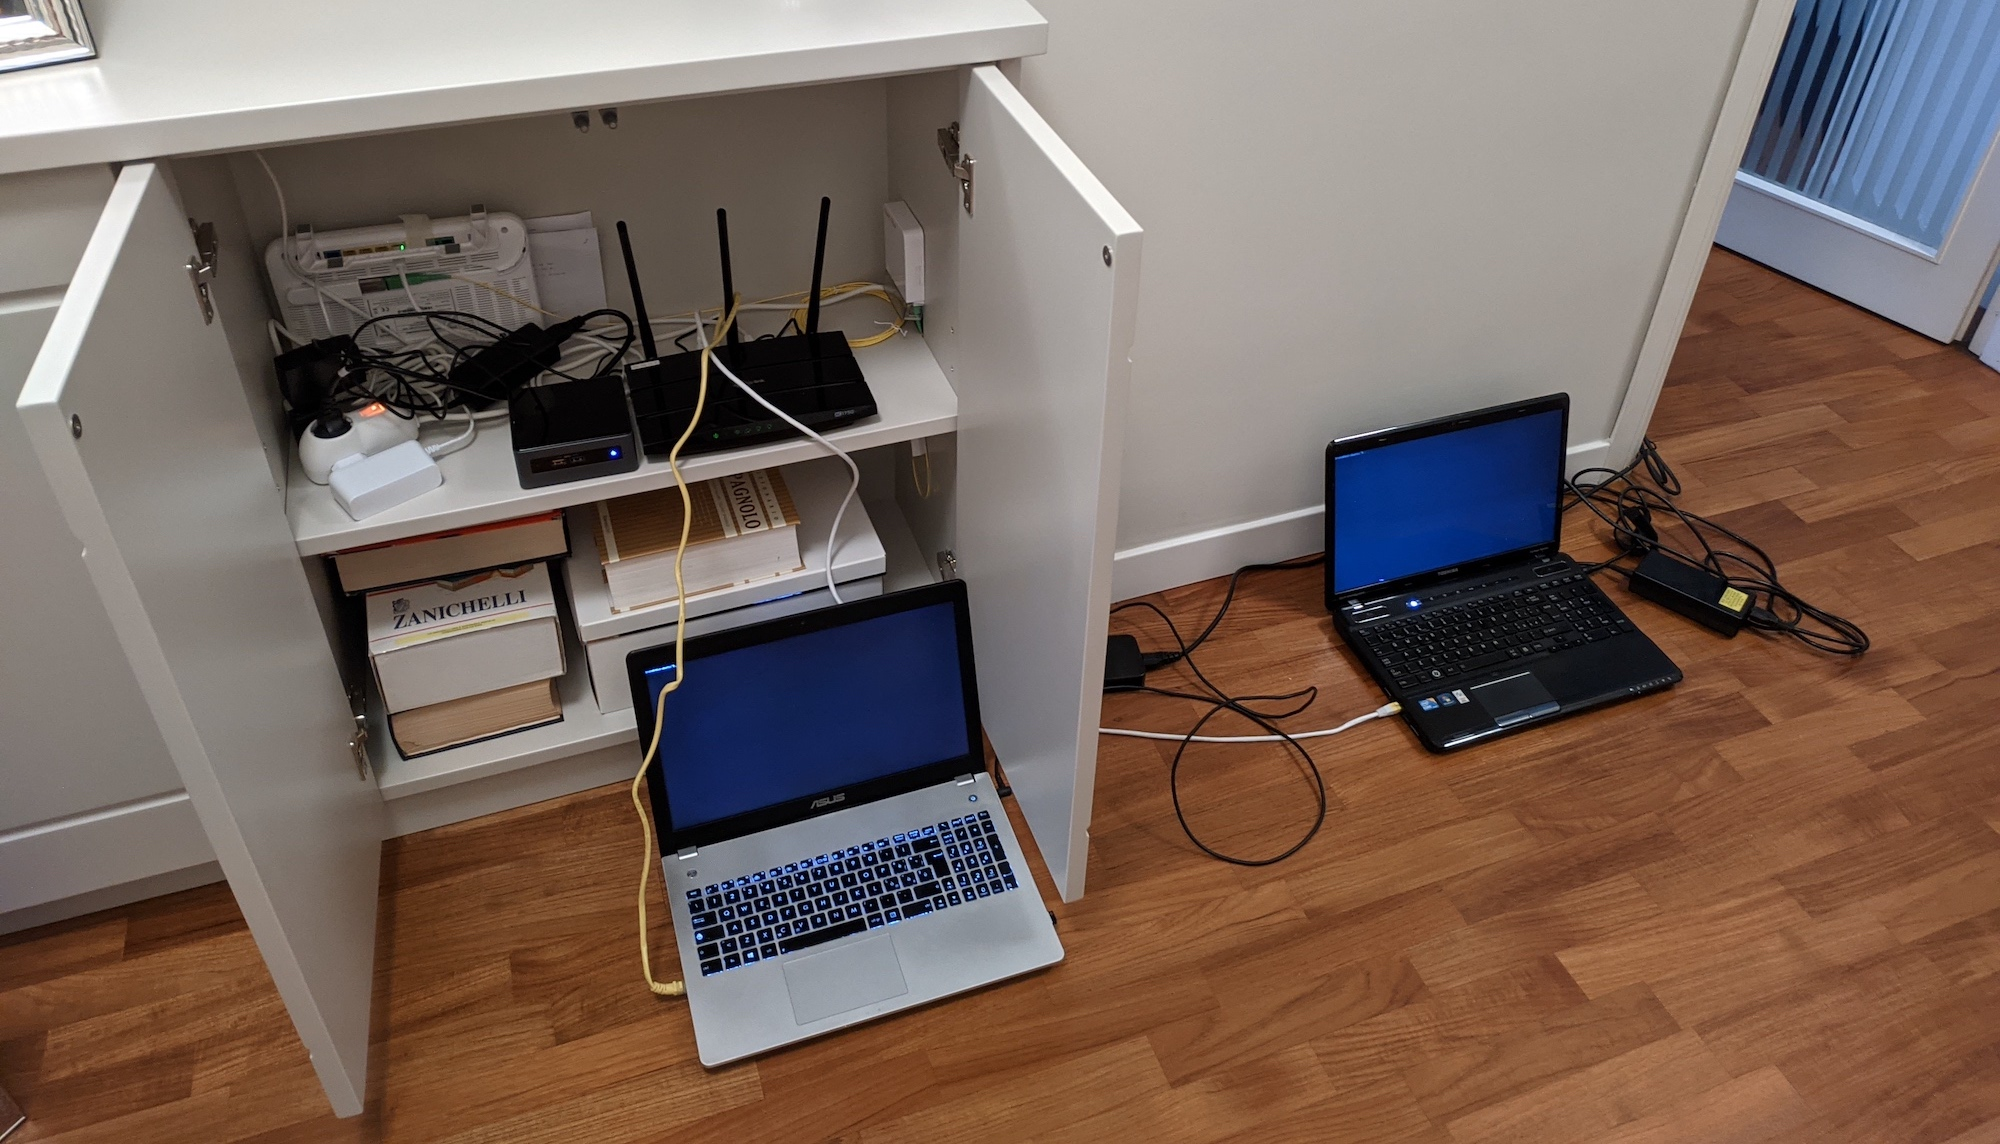
\includegraphics[width=0.85\textwidth]{figures/MPI-cluster.jpg}
\caption{Foto del cluster MPI domestico utilizzato}
\label{fig:MPI-cluster}
\end{figure}

\begin{table}[p]
\caption{Test di esecuzione seriale}
\label{tab:test-seriale}
\centering
\begin{tabular}{ccccccc}
\toprule
$N$ & $K$ & $e_\infty$ & $T_s$ & $E_s$ & $T_p$ & $E_p$ \\
\midrule
5000 & 4995 & \num{3.0433e-08} & \qty{0.634}{s} & \qty{25.372}{ns}
  & \qty{0.924}{s} & \qty{36.985}{ns} \\
10000 & 9989 & \num{7.6098e-09} & \qty{2.007}{s} & \qty{20.088}{ns}
  & \qty{2.680}{s} & \qty{26.829}{ns} \\
20000 & 19979 & \num{1.9026e-09} & \qty{6.874}{s} & \qty{17.204}{ns}
  & \qty{8.801}{s} & \qty{22.025}{ns} \\
40000 & 39959 & \num{4.7570e-10} & \qty{24.463}{s} & \qty{15.305}{ns}
  & \qty{39.832}{s} & \qty{24.920}{ns} \\
80000 & 79922 & \num{1.1867e-10} & \qty{91.212}{s} & \qty{14.266}{ns}
  & \qty{151.113}{s} & \qty{23.634}{ns} \\
\bottomrule
\end{tabular}
\end{table}

\begin{table}[p]
\caption{Test di strong scaling}
\label{tab:test-strong-scaling}
\centering
\begin{tabular}{ccccc}
\toprule
 & $M = 1$ & $M = 2$ & $M = 4$ & $M = 8$ \\
\midrule
$N$ & 80000 & 80000 & 80000 & 80000 \\
$K$ & 79922 & 79922 & 79922 & 79922 \\
\midrule
$W = 64$ & \qty{149.270}{s} & \qty{103.719}{s}
  & \qty{69.960}{s} & \qty{55.225}{s} \\
$W = 512$ & \qty{150.657}{s} & \qty{109.203}{s}
  & \qty{73.699}{s} & \qty{55.598}{s} \\
\midrule
Efficienza & 1 & 0.72 & 0.53 & 0.34 \\
\bottomrule
\end{tabular}
\end{table}

\begin{table}[p]
\caption{Test di weak scaling}
\label{tab:test-weak-scaling}
\centering
\begin{tabular}{ccccc}
\toprule
 & $M = 1$ & $M = 2$ & $M = 4$ & $M = 8$ \\
\midrule
$N$ & 20000 & 40000 & 80000 & 160000 \\
$K$ & 19979 & 39959 & 79922 & 159855 \\
\midrule
$W = 1$ & \qty{8.731}{s} & \qty{23.257}{s}
  & \qty{75.329}{s} & \qty{193.271}{s} \\
$W = 8$ & \qty{8.732}{s} & \qty{22.638}{s}
  & \qty{74.146}{s} & \qty{183.533}{s} \\
$W = 128$ & \qty{8.808}{s} & \qty{22.653}{s}
  & \qty{72.284}{s} & \qty{182.961}{s} \\
$W = 1024$ & \qty{8.757}{s} & \qty{23.229}{s}
  & \qty{79.672}{s} & \qty{183.724}{s} \\
\bottomrule
\end{tabular}
\end{table}

\subsection{Descrizione del cluster MPI domestico}
Eseguire il programma \code{07-FDM-parallel.py} su un unico
nodo ci è sembrato un controsenso: a quel punto perché
dovremmo preferire MPI a un approccio di tipo shared-memory?
Per questo motivo abbiamo scelto di realizzare
un \emph{cluster giocattolo} collegando due computer
portatili tramite uno switch gigabit ethernet
(foto in Figura \ref{fig:MPI-cluster}). Il cluster viene
controllato in remoto tramite \code{ssh} da un terzo portatile
posto in un'altra stanza. La distribuzione e l'aggiornamento
dei sorgenti Python sui due nodi del cluster è gestita tramite
\code{git}. Il lancio dei processi in parallelo sui vari
core dei cluster è effettuato mediante il comando \code{mpirun}
fornito da Open MPI, un'implementazione di MPI ad alte
prestazioni e open source.

Con riferimento alla foto,
il primo nodo del cluster è quello di destra,
dotato di un processore i7-720QM (microarchitettura
Nehalem, 4 core fisici, frequenza base 1.6 GHz, 6 MB di cache L3)
e 4 GB di RAM (DDR3 1066 MHz, larghezza di banda 16.8 GB/s).
Il secondo nodo del cluster è quello di sinistra,
dotato di un processore i7-3630QM (microarchitettura Ivy Bridge,
4 core fisici, frequenza base 2.4 GHz, 6 MB di cache L3)
e 8 GB di RAM (DDR3 1600 MHz, larghezza di banda 25.6 GB/s).
%
Abbiamo installato su entrambi i nodi una versione aggiornata
di Ubuntu 20.04 LTS; in questo modo ci siamo assicurati
che i due nodi eseguissero la stessa versione di Open MPI
(alcuni test preliminari avevano dato problemi a causa
di versioni diverse).

Abbiamo eseguito tre tipi di test: un test di esecuzione
seriale, un test sulle proprietà di strong scaling del codice
e infine un test sulle proprietà di weak scaling.

\subsection{Test di esecuzione seriale}
Nel primo test abbiamo misurato la differenza nel tempo
di esecuzione tra il programma \code{06\_FDM\_serial.py}
e il programma \code{07\_FDM\_parallel.py}
limitato a un solo processo ($M = 1$): in questo modo
abbiamo stimato l'overhead introdotto da MPI.
%
La Tabella \ref{tab:test-seriale} riporta i tempi di esecuzione
per valori di $N$ crescenti, da 5000 a 80000.
La tolleranza $\delta$ è fissata in ogni caso a $10^{-12}$.
Entrambi i programmi sono stati eseguiti sul primo
nodo del cluster.
Le colonne $T_s, T_p$ riportano i tempi di esecuzione totale
delle implementazioni seriale e parallela, rispettivamente,
mentre le colonne $E_s, E_p$ riportano i tempi di esecuzione
normalizzati rispetto al numero di incognite $N$ e al numero
di iterazioni $K$ effettuate per arrivare in convergenza,
come spiegato nel paragrafo 1.4.

Osserviamo che i tempi di esecuzione aumentano un po'
meno che quadraticamente rispetto a $N$; dato che
$K \approx N$, sarebbe lecito aspettarsi un andamento
esattamente quadratico. Il motivo è che al crescere
di $N$ aumenta l'efficienza del metodo, perché il programma
(sia seriale che parallelo con $M = 1$) passa relativamente più
tempo nelle routine vettoriali OpenBLAS
(sicuramente molto ben ottimizzate) rispetto al resto
del codice. Il tempo di esecuzione normalizzato, misurato dai
valori nelle colonne $E_s$ e $E_p$, sembra stabilizzarsi
intorno a $N = 80000$ nel caso seriale e $N = 20000$ nel
caso parallelo con $M = 1$.
L'errore $e_\infty$ tende a zero come $h^2$, esattamente
come previsto dalla teoria del metodo delle differenze finite.
Per quanto riguarda l'overhead introdotto da MPI, questo
è approssimativamente il 50\% del tempo di esecuzione,
almeno per i valori di $N$ testati. In realtà ci aspettiamo
che per $N \to \infty$ il rapporto $T_p/T_s$ tenda a 1,
ma non siamo riusciti a osservare questo comportamento.

\subsection{Test di strong scaling}
Nel secondo test abbiamo misurato il tempo di esecuzione
del programma \code{07\_FDM\_parallel.py}
all'aumentare del numero di processi $M$ mantenendo fisso
a 80000 il numero di incognite $N$ (test di \emph{strong scaling}).
La Tabella \ref{tab:test-strong-scaling} riporta i tempi
di esecuzione per $M = 1,2,4,8$. Nel caso $M \leq 4$,
tutti i processi sono stati lanciati su un unico nodo,
il primo, mentre per $M = 8$ i primi 4 processi sono stati
lanciati sul primo nodo e gli altri 4 processi sul secondo nodo.
Ribadiamo che non abbiamo fatto uso di load balancing,
ma dato che il secondo nodo è più potente del primo possiamo
supporre che le misure nel caso $M = 8$ siano equivalenti a quelle
che avremmo potuto ottenere su un cluster con il secondo nodo
uguale al primo (le prestazioni in eccesso sono semplicemente
sprecate). La tolleranza $\delta$ è fissata in ogni caso a $10^{-12}$.

Osserviamo che 	all'aumentare del numero di processi il tempo
di esecuzione effettivamente diminuisce, tuttavia l'efficienza
della parallelizzazione, definita dalla formula $T_s/(MT_p)$,
cala drasticamente. Ci siamo chiesti se la colpa fosse delle
operazioni di halo exchange, ma anche aumentando $W$
(in modo da rendere meno frequenti gli scambi) abbiamo
ottenuto risultati simili. Ipotizziamo quindi che
le operazioni di comunicazione collettiva \code{Allreduce()}
richieste dai prodotti scalari abbiano anch'esse
un costo significativo. Purtroppo, a differenza dell'halo
exchange, non è possibile raggruppare queste operazioni
per renderle meno frequenti. Riguardo alla rete gigabit ethernet,
questa non sembra essere il collo di bottiglia del nostro programma.

\subsection{Test di weak scaling}
Nel terzo test abbiamo misurato il tempo di esecuzione
del programma \code{07\_FDM\_parallel.py}
all'aumentare del numero di processi $M$ e all'aumentare
proporzionale di $N$ (test di \emph{weak scaling}).
Come costante di proporzionalità abbiamo scelto 20000,
in modo che $N = 20000 M$.
La Tabella \ref{tab:test-weak-scaling} riporta i tempi
di esecuzione per $M = 1,2,4,8$. Riguardo alla corrispondenza
tra rank e nodi e all'assenza di load balancing, valgono
le stesse considerazioni del test precedente.
La tolleranza $\delta$ è fissata in ogni caso a $10^{-12}$.

Osserviamo che, a parità di $N$, i tempi di esecuzione
diminuiscono all'aumentare di $M$, come si
evince dal confronto con la Tabella \ref{tab:test-seriale},
tuttavia i tempi sono ben lontani dall'essere lineari
rispetto a $M$. L'unico dato incoraggiante è che, per
valori grandi di $W$, il tempo di esecuzione per $M = 8$
è di poco maggiore del doppio di $M = 4$. Ipotizziamo quindi
che per valori ancora maggiori di $N$ si potrebbe osservare
una dipendenza lineare tra il tempo di esecuzione del
programma e il numero di processi $M$.

\subsection{Conclusioni}
L'obiettivo di parallelizzare il metodo del gradiente
coniugato è stato raggiunto: la versione parallela del programma
fornisce gli stessi errori della versione seriale (a conferma della
sua correttezza) e richiede meno tempo per essere eseguita
all'aumentare del numero di processi nella sessione MPI,
anche quando i processi sono divisi tra nodi diversi
all'interno del nostro cluster domestico.
Purtroppo i dati raccolti sulle proprietà di strong e weak
scaling non sono del tutto soddisfacenti.
Siamo consapevoli che avremmo potuto raccogliere
dati più affidabili se avessimo eseguito più volte ciascun test
(per farne delle statistiche) e se avessimo avuto controllo di
aspetti quali core pinning, dynamic frequency scaling
e thermal throttling dei processori. Ci riteniamo
tuttavia soddisfatti vista la semplicità del codice scritto
e l'uso di un cluster giocattolo.

%\printbibliography[heading=bibintoc, title={Bibliography}]

\end{document}




















